% !TEX root = ../main.tex
%

\section{Results}
\label{sec:results}

\subsection{Main findings}

\begin{enumerate}[nosep, noitemsep]
    \item Unmoderated discussions exhibit significantly higher toxicity and lower \ac{AQ} (Fig.~\ref{fig::toxicity_aq_stats}) (ANOVA\footnote{The large size and balanced nature of our dataset allows the use of parametric tests.} $p<.000$).

    \item  While the Moderation and Facilitation Guidelines slightly improve \ac{AQ} relative to baselines, their impact is marginal (Fig.~\ref{fig::toxicity_aq_stats}). Notably, these strategies do not reduce toxicity more effectively than the “No Instructions” baseline and perform worse than the “Rules Only” strategy.

    \item Toxicity and \ac{AQ} generally improve over time under all strategies when compared to unmoderated discussions, indicating a limited, but consistent restraining effect by the \ac{LLM} moderators over time (Table~\ref{tab:timeseries}).

    \item \ac{LLM} moderators intervene frequently throughout discussions (Fig.~\ref{fig::intervention_count}). \ac{LLM} user-agents exhibit atypical tolerance for excessive moderator interventions, whereas with human participants such repeated interventions often provoke irritation and increased toxicity \cite{schaffner_community_guidelines, make_reddit_great, proactive_moderation, cresci_pesonalized_interventions}.
\end{enumerate}


\begin{figure*}[t]
    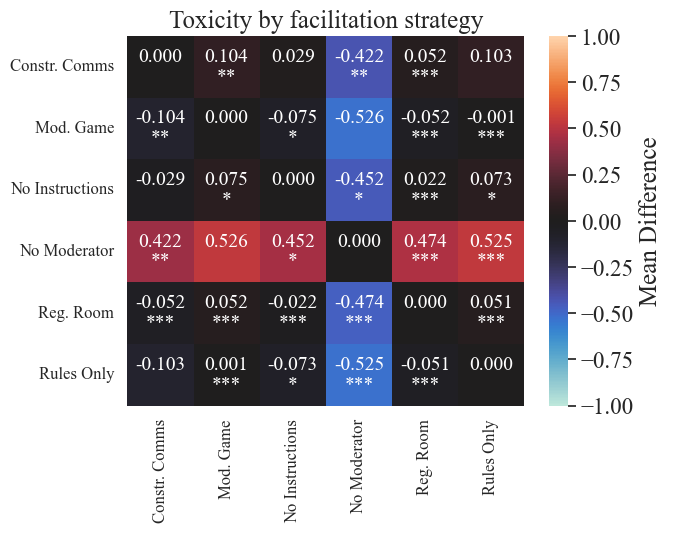
\includegraphics[width=0.48\linewidth]{toxicity_stats.png} \hfill
    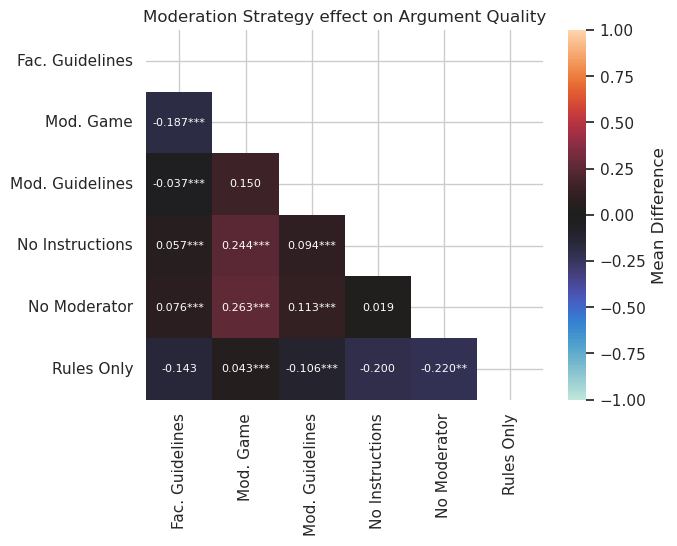
\includegraphics[width=0.48\linewidth]{argumentq_stats.png}
	\centering
	\caption{Mean difference of Toxicity (left) and \ac{AQ} (right) between each moderation strategy. $A[i, j] = 0.3^{***}$ indicates that the strategy $i$ leads to overall worse discussions (more toxicity/worse arguments) compared to $j$ for an average of $0.3$ annotation levels ($1-5$) with $p<0.001$. Each comparison is accompanied by pairwise student-t tests, in the form of significance asterisks.}
	\label{fig::toxicity_aq_stats}
\end{figure*}

\begin{figure}
	\centering
	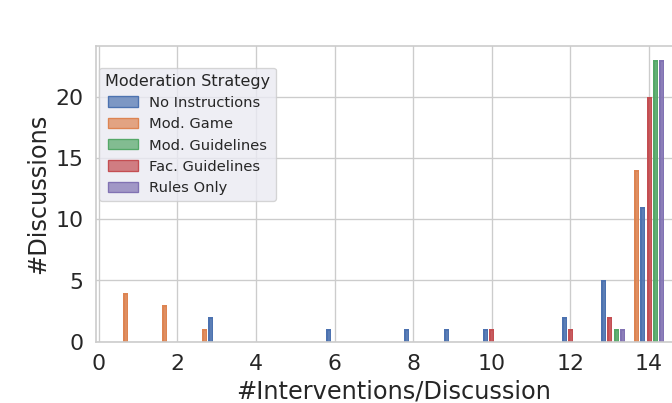
\includegraphics[width=\columnwidth]{intervention_count.png}
	\caption{Histogram of interventions by \ac{LLM} moderators. The maximum number of interventions is $14$.}
	\label{fig::intervention_count}
\end{figure}

\begin{table}[htbp]
    \centering
    \begin{tabular}{lll}
        \toprule
        \textbf{Variable} & \textbf{Toxicity} & \textbf{Arg.Q.} \\
        \midrule
        Intercept & 2.164\textsuperscript{***} & 2.113\textsuperscript{***} \\
        Fac. Guid. & -0.230\textsuperscript{***} & -0.007 \\
        Mod. Guid. & -0.277\textsuperscript{***} & -0.107\textsuperscript{*} \\
        \ac{RL} Game & -0.435\textsuperscript{***} & -0.282\textsuperscript{***} \\
        No Instructions & -0.426\textsuperscript{***} & -0.213\textsuperscript{***} \\
        Rules Only & -0.461\textsuperscript{***} & -0.305\textsuperscript{***} \\
        time & -0.012\textsuperscript{**} & -0.012\textsuperscript{**} \\
        Fac. Guid$\times$time & -0.023\textsuperscript{***} & -0.024\textsuperscript{***} \\
        Mod. Guid$\times$time & -0.023\textsuperscript{***} & -0.011\textsuperscript{*} \\
        \ac{RL} Game$\times$time & -0.011\textsuperscript{*} & 0.003 \\
        No Instructions$\times$time & -0.003 & 0.003 \\
        Rules Only$\times$time & -0.008 & -0.002 \\
        \bottomrule
    \end{tabular}
    \small
    $\cdot p<0.1$, \textsuperscript{*} $p<0.05$, \textsuperscript{**} $p<0.01$, \textsuperscript{***} $p<0.001$
    \normalsize
    \caption{OLS Regression Coefficients for Toxicity ($Adj. R^2=0.054$) and \ac{AQ} ($Adj. R^2=0.016$). \textit{“Time”} denotes dialogue turn, reference factor is \textit{“No moderator”}.}
    \label{tab:timeseries}
\end{table}



\subsection{Ablation study}
\label{ssec:results:ablation}

We test the effects of our proposed methodology by running $8$ synthetic discussions using the Qwen 2.5 model, and comparing their \textit{diversity} scores (Section \ref{ssec:methodology:diversity}) with our original dataset, as well as with human discussions. We use the Cornell eRulemaking “Regulation Room” dataset \footnote{\url{http://archive.regulationroom.org}}, from which we extract all comments from all initiatives. 

% Any opinions, findings, and conclusions or recommendations expressed in this material are those of the author(s) and do not necessarily reflect the views of the CeRI (Cornell e-Rulemaking Initiative)


\subsubsection{Models}

Among examined models, Qwen 2.5 exhibits the highest observed diversity, followed by Mistral Nemo and LLaMa 3.1 (Fig.~\ref{fig::diversity}). Notably, the Mistral model approximated the comment length of human discussions the best (Fig.~\ref{fig::comment_length}). While maximizing diversity should not be the primary objective (a discussion with maximum diversity may indicate that the participants do not engage with each other), these results suggest that large and intensely aligned \acp{LLM} such as LLaMa may struggle to replicate authentic human conversational dynamics compared to other models, as also reported by \citep{Park2023GenerativeAI}.

Alternatively, LLaMa's longer comments (Fig.~\ref{fig::comment_length}) may have caused the higher diversity scores. We find a qualitatively and statistically significant positive correlation ($\textit{diversity} = 2.38\mathrm{e}{-05} \times \textit{\#words} \times \textit{is\_synthetic} + 0.9030, Adj. R^2=0.202$) between the length of \textit{synthetic} discussions and their diversity score. There is no such significance for human texts ($p=0.775$).


\subsubsection{Turn taking}

We assess three methods for controlling user turns: Round Robin (placing each participant in a predetermined queue), Random Selection, and our own approach (Section~\ref{ssec:experimental:turn}). Although no single function fully replicates human diversity (Fig.~\ref{fig::diversity}), both traditional methods yield discussions with extremely high diversity scores, deviating significantly from human norms. Our proposed algorithm improves synthetic conversations by reducing this divergence, demonstrating meaningful positive effects on data quality that cannot be attributed to comment length alone (Fig.~\ref{fig::comment_length}).


\subsubsection{Prompting}

We run discussions where user-agents (1) are not assigned \acp{SDB}, (2) are not assigned roles, and (3) are given a basic instruction prompt (see Appendix~\ref{sssec:appendix:actors}). Fig.~\ref{fig::diversity} demonstrates that, while our approach (using roles, \acp{SDB}, and our improved instruction prompt) is not enough to create synthetic discussions with similar diversity as human discussions, removing any of its aspects leads to a significant divergence. This divergence is similar to the one observed when changing the turn taking function, and can similarly not be attributed to differences in comment length (Fig.~\ref{fig::comment_length}).

Interactions involving “Troll” user-agents, guided by our finetuned instruction prompt, resulted in more toxic comments and reduced \ac{AQ} (Student-t test: $p<.000$) among other users (Fig.~\ref{fig::boxplots})\footnote{This experiment was conducted with a moderator supplied with the “No Instructions” strategy.}. This effect is absent when we remove explicit instructions to react to toxic posts, although notably, the absence of these instructions still leads to a decrease in \ac{AQ}. Thus, our finetuned instruction prompts are necessary to induce behavior which our moderators can work on improving.

\begin{figure}[t]
    \centering
    \begin{tabular}{cc}
            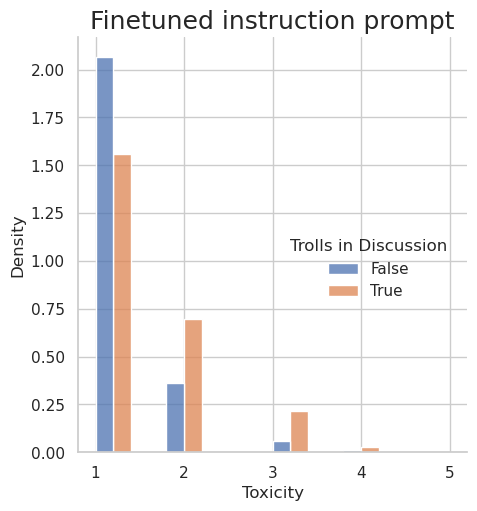
\includegraphics[width=0.45\columnwidth]{boxplot_toxicity_original.png} &
            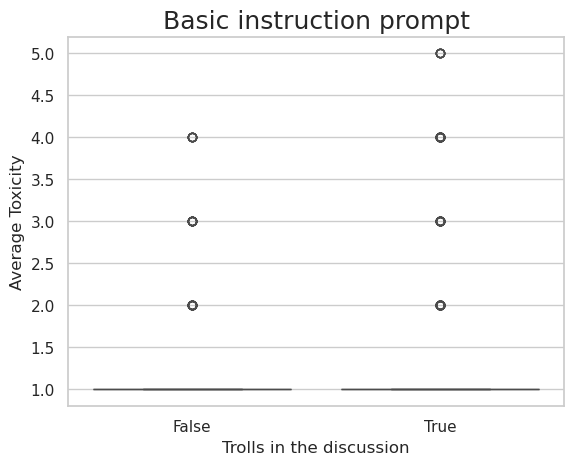
\includegraphics[width=0.45\columnwidth]{boxplot_toxicity_basic.png} \\ 
            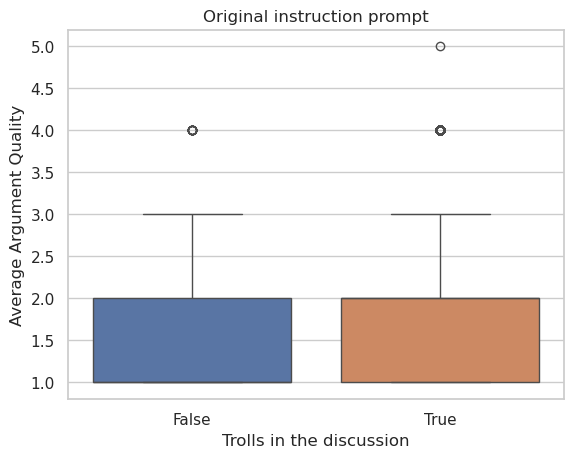
\includegraphics[width=0.45\columnwidth]{boxplot_aq_original.png} &        
            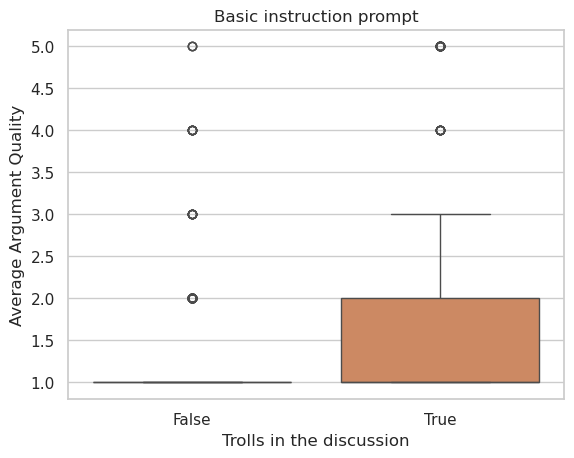
\includegraphics[width=0.45\columnwidth]{boxplot_aq_basic.png}
    \end{tabular}
    \caption{Toxicity (upper row) and \ac{AQ} (bottom row) of synthetic discussions, excluding comments by troll user-agents. First column includes synthetic discussions with our finetuned instruction prompts, second column uses the basic ablation instruction prompt. Less is better.}
    \label{fig::boxplots}
\end{figure}

\begin{figure*}[t]
    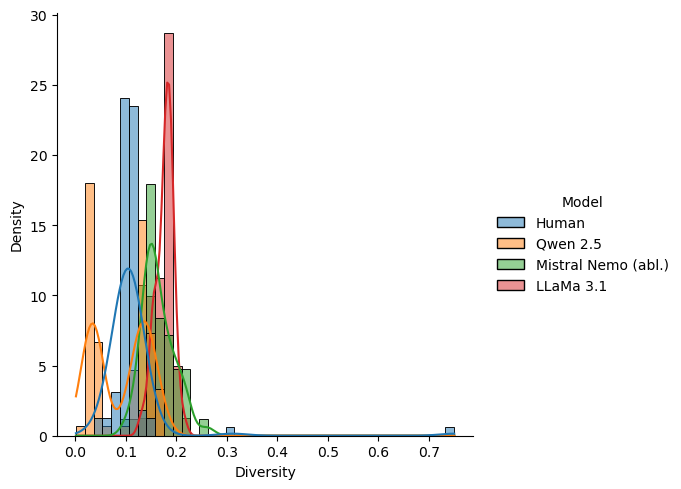
\includegraphics[width=0.30\linewidth]{rougel_model.png} \hfill
    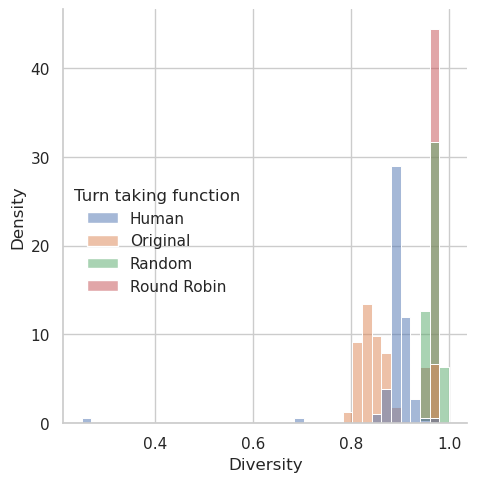
\includegraphics[width=0.30\linewidth]{rougel_turns.png}
    \hfill
    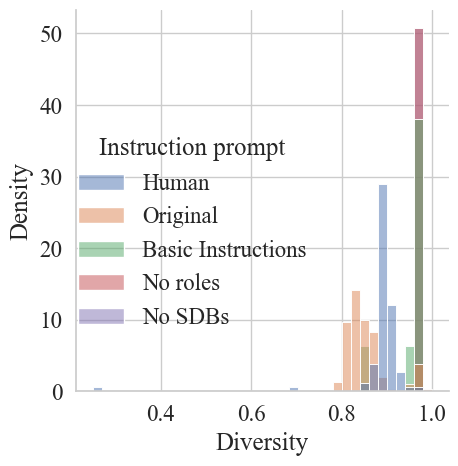
\includegraphics[width=0.30\linewidth]{rougel_prompts.png}
	\centering
	\caption{Diversity (Section~\ref{ssec:methodology:diversity}) distribution for each discussion by model (Section~\ref{ssec:experimental:model}), turn-taking function $u$ (Section~\ref{ssec:experimental:turn}), and prompting function $\phi$ used (Section~\ref{ssec:experimental:prompts}).}
	\label{fig::diversity}
\end{figure*}

\begin{figure*}[t]
    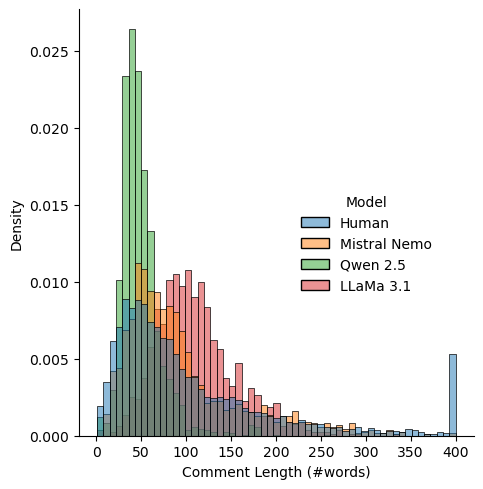
\includegraphics[width=0.30\linewidth]{comment_len_model.png} \hfill
    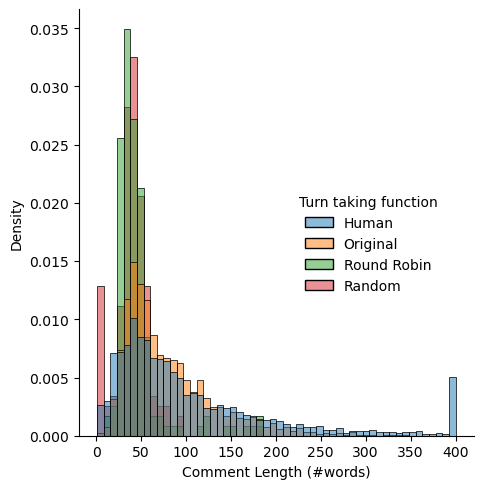
\includegraphics[width=0.30\linewidth]{comment_len_turns.png}
    \hfill
    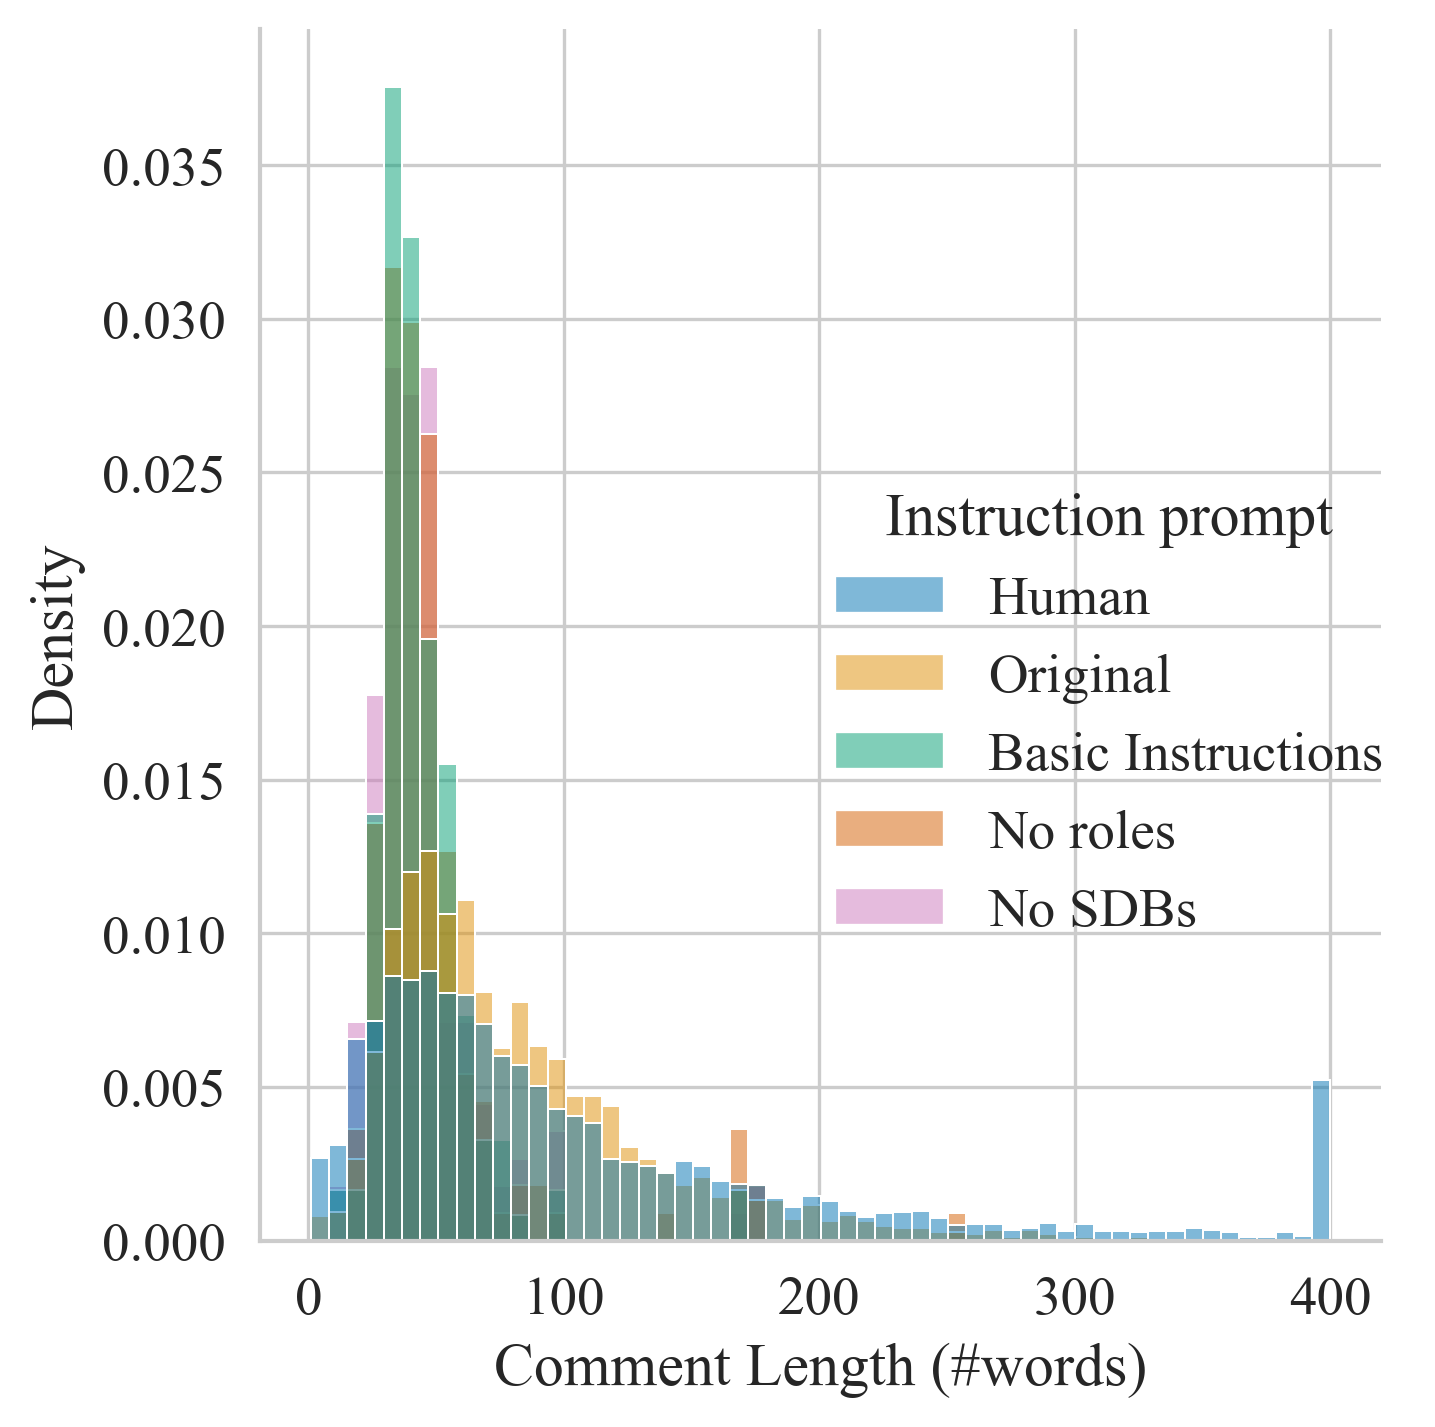
\includegraphics[width=0.30\linewidth]{comment_len_prompts.png}
	\centering
	\caption{Comment length for each discussion by model (Section~\ref{ssec:experimental:model}), turn-taking function $u$ (Section~\ref{ssec:experimental:turn}), and prompting function $\phi$ used (Section~\ref{ssec:experimental:prompts}). For ease of comparison, comments above $400$ words are marked at the end of the x-axis.}
	\label{fig::comment_length}
\end{figure*}



